\subsubsection{Drucksensor}
In der Teststation gibt es eine Vorrichtung, um ein Vakuum zu erzeugen. Durch dieses Vakuum kann der integrierte barometrischer Drucksensor auf dem CubeSat getestet werden. Der Drucksensor in der Kammer wird dazu verwendet, einen Vergleich zwischen Testkammer und Satellit herzustellen.\\
\vspace{3mm}
Es wurde der Drucksensor BMP180\autocite{BMP180} verwendet. Er befindet sich in der Testkammer, hat jedoch keinen fixen Platz. Der Sensor kann je nachdem, ob ein Vakuum erzeugt wird oder nicht, platziert werden. Der BMP180 hat 4 Pins die über die PCB angeschlossen und mit dem \raspi verbunden. werden.\\
\vspace{3mm}
\begin{table}[h]
    \centering
    \begin{tabular}{ | c | c | } 
  \hline
   Vin & 5 Volt\\ 
  \hline
   GND & Ground\\ 
  \hline
   SDA & GPIO3 \\ 
  \hline
   SCL & GPIO5 \\ 
  \hline
\end{tabular}
    \caption{Pinbelegung Drucksensor}
\end{table}
\vspace{3mm}
Um den Sensor verwenden zu können, muss auch hier eine Bibliothek heruntergeladen werden. Diese wird von Adafruit bereitgestellt. Mit folgendem Befehl kann die Bibliothek\autocite{BMP180bib} heruntergeladen werden.
\begin{verbatim}
pip install circuitpython-bmp180
\end{verbatim}
Die Suche nach einer geeigneten Bibliothek war nicht einfach, da die meisten Repository archiviert wurden. In einigen Dokumenten wird auch angegeben, dass der Drucksensor BMP180 gar nicht mehr hergestellt wird.\\
\vspace{3mm}
\begin{figure}[H]
    \centering
    \begin{subfigure}[b]{0.7\textwidth}
        \centering
        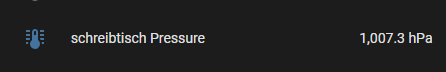
\includegraphics[width=\textwidth]{image/druckvergleich.png}
        \caption{Messung über Wetterstation}
        \label{fig:bild1}
    \end{subfigure}
    \hfill
    \begin{subfigure}[b]{0.5\textwidth}
        \centering
        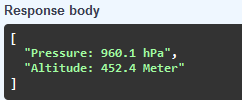
\includegraphics[width=\textwidth]{image/druckausgabe.png}
        \caption{Messung mit Drucksensor}
        \label{fig:bild2}
    \end{subfigure}
    \caption{Druckmessungen}
    \label{fig:zwei_bilder}
\end{figure}
Die oben angeführten Druckmessungen, wurden beide in Wolfurt durchgeführt. Der Druck in Abbildung (a), wurde mit einer Netatmo Wetterstation\autocite{Netatmo} gemessen. In Abbildung (b), wurde der BMP180 Drucksensor verwendet, um den Druck zu ermitteln. Die Werte stimmen einigermaßen überein. Auch die Meereshöhe kann mit dem BMP180 angezeigt werden. Wolfurt liegt auf einer Meereshöhe von 434 m. Der Sensor zeigt eine Meereshöhe von 452 Metern an. Da dieser Wert nicht genau mit dem tatsächlichen Wert über einstimmt, kann eine Kalibrierung durchgeführt werden. Dies erfolgt durch eine Anpassung an der Berechnung im Code.\\
\vspace{3mm}
Der Codeabschnitt für das Testprogramm befindet sich im Kapitel  \ref{sec:Testprogramm Drucksensor}. Das Programm für die API ist im Kapitel \ref{sec:API-Druck}.